%!TEX root=Principal.tex
\chapter{TECNOLOGIAS E TESTES}
\label{cap:tecnologiaetestes}
Esse capítulo apresentará as tecnologias e equipamentos utilizados para o desenvolvimento e o cenário de teste considerado para validação do processo de interação entre humanos e robôs proposto por essa tese.

\section{O Robô}
\label{sec:robo}
O robô utilizado no desenvolvimento da tese é o PeopleBot~\footnote{PeopleBot - http://www.mobilerobots.com/researchRobots/PeopleBot.aspx} fabricado pela ActivMedia Robotics. Ele é um robô móvel com direção diferencial, ou seja, possui duas rodas motorizadas e uma roda castor que auxilia em seu equilíbrio. O projeto do PeopleBot tem foco em pesquisas e serviços que envolvem interação humano-robô. Com esse objetivo, ele foi desenvolvido com uma altura de 112 cm (centímetros). Além disso, o PeopleBot também possui uma garra pequena que tem sua movimentação apenas na direção vertical. A figura~\ref{fig:peoplebot} apresenta o robô PeopleBot.

\begin{figure}[ht!]
	\centering
	\begin{minipage}{\textwidth}
		\caption{Robô ActivMedia Robotics PeopleBot.}
		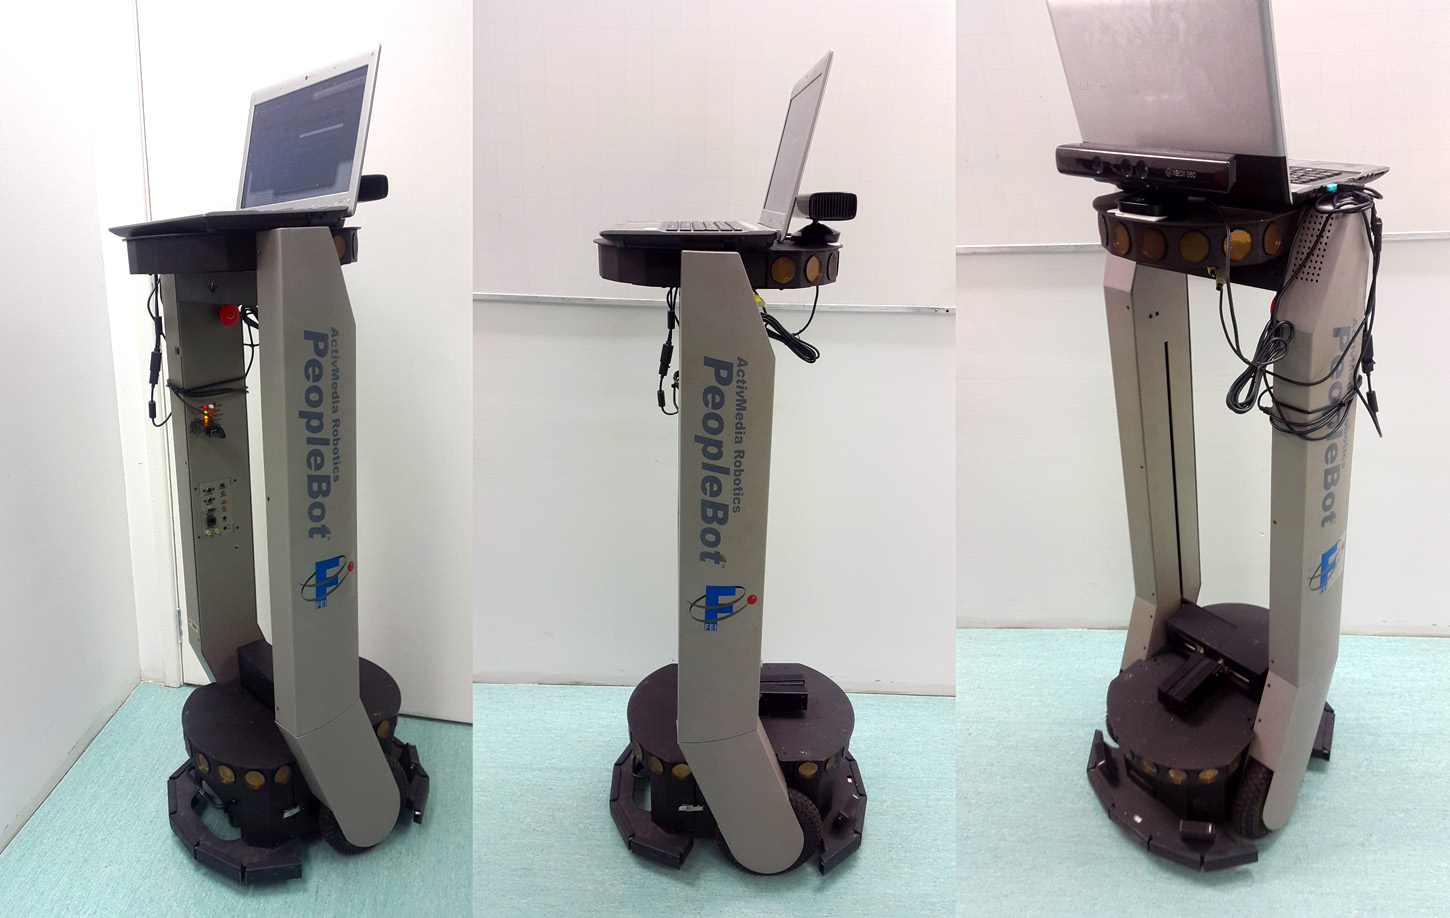
\includegraphics[width=\textwidth]{peoplebot.jpg}
		\smallcaption{Fonte: Autor.}
		\label{fig:peoplebot}
	\end{minipage}
\end{figure}

Como a garra do PeopleBot é curta e não permite muita destreza na manipulação de objetos e gestos, além de possuir poucos graus de liberdade, foi adicionado um novo manipulador. O projeto do manipulador foi desenvolvido com o intuito de auxiliar a manipulação de objetos a uma certa distância e execução de gestos durante interações com pessoas. O projeto atende pesquisas com foco em prestação de serviços domésticos e cuidados pessoais. O desenho que ilustra o manipulador desenvolvido é apresentado através da figura~\ref{fig:manipulador}.

\begin{figure}[ht!]
	\centering
	\begin{minipage}{0.6\textwidth}
		\caption{Projeto do Novo Manipulador do PeopleBot.}
		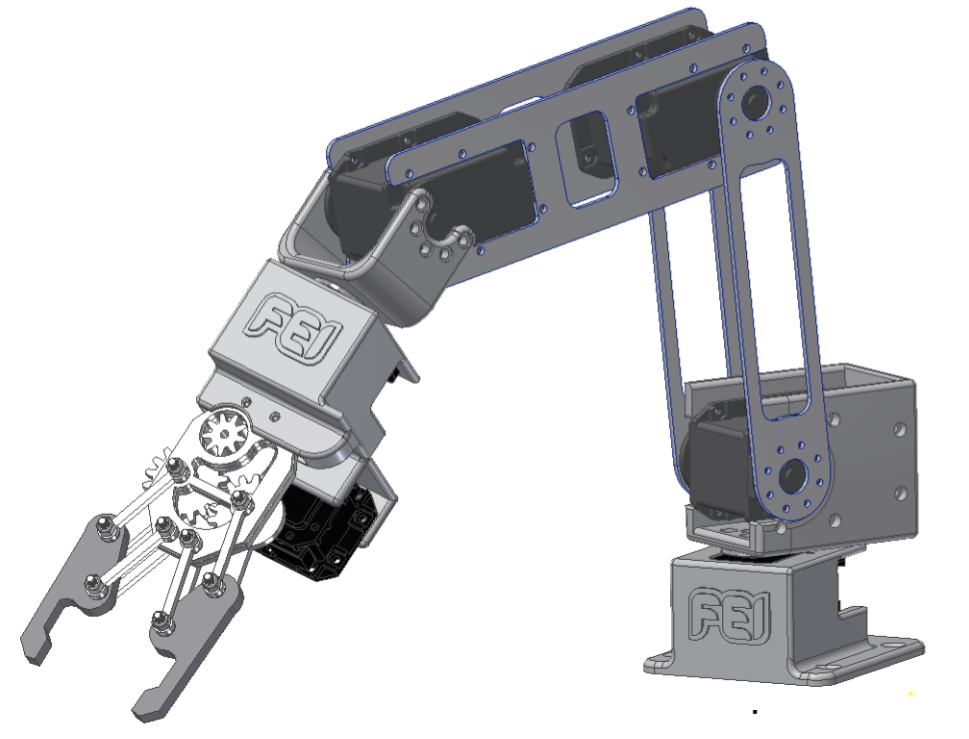
\includegraphics[width=\textwidth]{manipulador.png}
		\smallcaption{Fonte: Autor.}
		\label{fig:manipulador}
	\end{minipage}
\end{figure}

O novo manipulador foi construído de maneira que os movimentos sejam próximos do braço humano. Além do manipulador, também foi acoplado um \emph{tablet} para que seja possível atribuir face ao robô e consequentemente expressões faciais, deixando a interação mais amigável. O projeto da cabeça do robô é apresentado na figura~\ref{fig:judithhead}.

\begin{figure}[ht!]
	\centering
	\begin{minipage}{0.4\textwidth}
		\caption{Projeto da Cabeça para o PeopleBot.}
		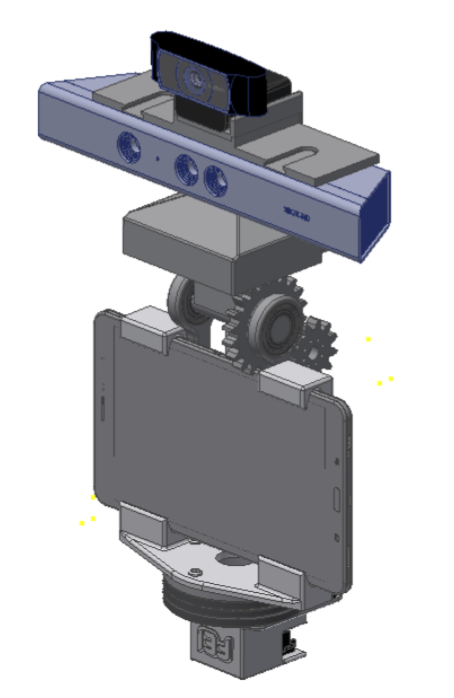
\includegraphics[width=\textwidth]{judith_head.png}
		\smallcaption{Fonte: Autor.}
		\label{fig:judithhead}
	\end{minipage}
\end{figure}

O projeto da cabeça foi preparado para acomplar alguns alguns sensores como o Microsoft\textregistered\ Kinect\textregistered\ , o ASUS\textregistered\ Xtion\textregistered\ e webcams, para tarefas que envolvam nuvem de pontos de profundidade e visão computacional. Sensores como lasers e microfones também foram instalados para melhorar a captura de informações sobre o ambiente e interagir melhor com a pessoa.

\section{Arquitetura do Software}
\label{sec:arquitetura}
A arquitetura construída para o software do robô foi feita em camadas. Existem 3 camadas principais, que definem a arquitetura do robô. A primeira camada contém os estados que compõem as máquinas de estados que auxiliam o robô nas tarefas a serem realizadas. Basicamente, ela conduz as ações e comandos que o robô tem como interface com o usuário durante a interação.

A segunda camada é responsável pelo processamento dos processos de \emph{subscribers} e \emph{publishers}, conforme o recomendado pelo \emph{Robot Operating System}~(ROS)~\footnote{http://www.ros.org/}. Eles fazem a interface entre sensores e atuadores, através de seus \emph{drivers}, e também com os algoritmos de visão computacional, de aprendizado de máquina e de planejamento. O processamento desses algoritmos, de sensores com grande volume de informação como o Kinect e serviços que auxiliam o controle do manipulador são encontrados na terceira camada.

Como toda a implementação do software foi feita com base no ROS, os pacotes foram construídos de maneira separada. Sendo assim, os códigos fontes ficaram agrupados de acordo com as habilidades necessárias para o robô realizar as tarefas e também referentes ao mesmo tipo de objetivo. Todo o código fonte criado para execução dos testes dessa tese, encontram-se disponível através do endereço \url{https://github.com/amasiero/approach_control}, na ferramente de controle de versão em código aberto, GitHub. O código foi testado com duas bases robóticas, o PeopleBot da Pioneer e o youBot da Kuka.

\subsection{Bibliotecas}
\label{sec:bibliotecas}
Para auxiliar no desenvolvimento da tese, algumas bibliotecas e softwares foram utilizados. O primeiro, conforme dito na seção~\ref{sec:arquitetura}, foi o ROS que é um \emph{framework} para desenvolvimento de software em robôs. Ele roda sobre o Ubuntu Linux, que no caso da tese foi utilizado a versão 14.04, com o ROS versão Indigo.

A biblioteca que gerencia a máquina de estados criada para execução das tarefas é o SMACH~\footnote{http://wiki.ros.org/smach}. Ele possibilita a criação e realiza o gerenciamento dos estados durante a execução das ações do robô. Para reconhecimento de voz a biblioteca utilizada foi o Dragonfly Speech Recognition~\footnote{https://pypi.python.org/pypi/dragonfly/0.6.5}. Bibliotecas como o OpenCV~\footnote{http://opencv.org/}, PyOpenni~\footnote{https://github.com/jmendeth/PyOpenNI} e MoveIt!~\footnote{http://moveit.ros.org/} foram utilizados para percepção e interação com o ambiente e também com o usuário.

Todos os pacotes desenvolvidos utilizaram a linguagem de programação Python, que possibilitou diversas facilidades na implementação dos códigos e integração das camadas dos pacotes no ROS. Para criação e teste da rede bayesiana proposta utilizou-se o \emph{framework} SamIam~\footnote{http://reasoning.cs.ucla.edu/samiam/}, que realiza os cálculos de todas as probabilidades de uma consulta a rede de maneira objetiva e com um bom desempenho computacional.

\section{Cenário de Teste} %REFAZER OS TEXTOS DESSA SEÇÃO
\label{sec:cenario}
Antes de descrever o cenário de teste, é importante mencionar que todo o procedimento para a execução foi aprovado por um comitê de ética, e pode ser consultado a partir do identificador CAAE: 70057117.0.0000.5508. O teste é realizado em um cenário simulando um residência, conforme apresentado na figura~\ref{fig:cenario}.

\begin{figure}[ht!]
	\centering
	\begin{minipage}{\textwidth}
		\caption{Cenário para teste de interação com o robô.}
		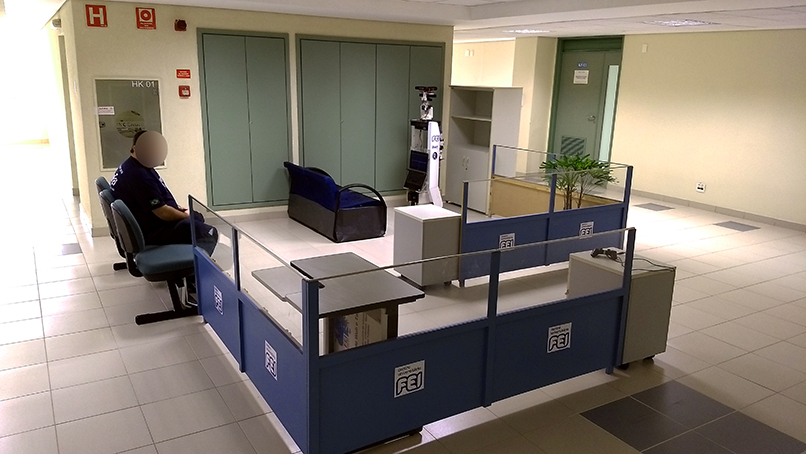
\includegraphics[width=\textwidth]{cenario.jpg}
		\smallcaption{Fonte: Autor.}
		\label{fig:cenario}
	\end{minipage}
\end{figure}

\subsection{Objetivo}

O robô deve se comportar durante a aproximação de qualquer agente fazendo com que este confortável independente da aparência que o robô tenha e de maneira natural.

\subsection{Foco}

O foco do cenário é o aprendizado e generalização de uma aproximação do robô à uma pessoa ou um grupo de pessoas, nas posições, sentada ou em pé.

\subsection{Configuração para o Teste}

Para esse teste deverão ser considerados algumas possibilidades para o robô e também pessoas. Essas configurações podem ser mescladas entre si, atendendo qualquer possível combinação.

\subsubsection{Pessoa}

\begin{itemize}
	\item Única pessoa parada em pé a 4 metros a frente do robô. A pessoa não precisa necessariamente ficar olhando diretamente para o robô.
	\item Única pessoa sentada a 4 metros a frente do robô. A pessoa não precisa necessariamente ficar olhando diretamente para o robô. Ela poderá ler um livro ou revista, nessa configuração.
	\item Grupo de pessoas simulando uma conversa a 4 metros de distância a frente do robô. Neste caso todas as pessoas estarão em pé.
	\item Grupo de pessoas simulando uma sala de estar a 4 metros de distância a frente do robô. Neste caso poderá existir pessoas sentadas e em pé (paradas ou caminhando pelo ambiente).
\end{itemize}

O objetivo das configurações do grupo de pessoas acima é fazer com que o robô aprenda a se aproximar das diversas formações possíveis, permitindo assim uma melhor generalização do modelo aprendido.

\subsubsection{Robô}

\begin{itemize}
	\item O robô possui face que interage com a pessoa de acordo com suas próprias ações. Por exemplo, quando falar olá o robô apresenta uma face sorrindo. (Aprender quais as melhores expressões faciais para deixar o indivíduo confortável na aproximação do robô de acordo com as zonas de proximidades)
	\item O robô não possui face. (Validar se é possível um robô se aproximar de uma pessoa sem nenhum sinal social e deixar a pessoa confortável)
	\item O robô controla os gestos do manipulador ao se aproximar da pessoa. Neste caso ele pode ou não possuir uma face. (Aprender quais os melhores gestos para deixar o indivíduo confortável na aproximação do robô de acordo com as zonas de proximidades)
	\item O robô não controla os gestos do manipulador ao se aproximar da pessoa. Neste caso ele pode ou não possuir uma face. (Aprender quais os melhores gestos para deixar o indivíduo confortável na aproximação do robô de acordo com as zonas de proximidades)
	\item O robô não realiza gestos. Neste caso o robô pode ou não possuir o manipulador. (Validar se é possível um robô se aproximar de uma pessoa sem apresentar gestos com seu manipulador, ou sem ele, e deixar a pessoa confortável)
\end{itemize}

Para todos os casos de robôs, ele poderá apresentar ou não sinais de voz para interagir com a pessoa durante a aproximação.

\subsection{Tarefa}

Esse teste poderá ocorrer em um ambiente não controlado, onde existam pessoas não participantes, transitando pelo cenário, devido ao espaço necessário para execução do teste.

\begin{enumerate}
	\item \textbf{Início}: O robô é posicionado no cenário de maneira aleatória e aguarda o comando para início do teste.
	\item \textbf{Identificando a pessoa ou o grupo}: O robô deve rotacionar até encontrar o marcador feito com um QRCODE que identifica a pessoa ou o grupo que ele deve interagir.
	\item \textbf{Aproximando do objetivo}: Ao identificar o grupo que ele deve se aproximar, o robô inicia a aproximação. Antes do início do movimento em direção ao grupo, de maneira aleatória, ele poderá ou não emitir sons, apresentar faces e/ou executar gestos com seu manipulador.
	\item \textbf{Reações das pessoas}: Todas as reações das pessoas, durante a aproximação do robô, deverão ser armazenadas com o intuito de aprender se as ações executadas tornaram a aproximação mais confortável ao grupo.
	\item \textbf{Fim}: Será considerado o fim da tarefa, quando o robô permanecer em interação dentro do espaço pessoal para intimo, por 15 segundos ou em um tempo máximo de 5 minutos total da tarefa.
\end{enumerate}

\section{Seleção das Pessoas para o Teste}
\label{sec:perfistestes}
Para realizar os testes são priorizadas as pessoas que não tiveram nenhum contato prévio com robô ou com um contato mínimo. As pessoas possuem idades diversificadas, porém as preferências são por idosos e crianças. Alguns candidatos ao teste possuem medo declarado de robôs e neste caso o especialista ficará acompanhando o teste com uma maior proximidade para evitar problemas com o robô e principalmente com a pessoa.

Os integrantes da equipe que constrói o robô não serão consideradas como público ou registro oficial dos testes realizados nos dois cenários. Também são evitados a repetição dos candidatos entre os dois cenários com a tentativa de maximizar o resultado dos testes.
